\documentclass[../../main.tex]{subfiles}

\begin{document}

\section{Motivation}

Machine learning models have been immensely successful in variety of applications to generate predictions in data-driven domains such as computer vision, robotics, weather forecasting. While the success of these models is undeniable, they tend to lack the ability to understand the uncertainty in the predictions. This is a major drawback in the deployment of these models in real-world applications, for example, in weather forecasting,  the uncertainty of the prediction of the weather is arguably as valuable as the prediction itself. In this work, we aim to implement a model that is \textbf{uncertainty aware} whilst also possessing further desirable properties.

\section{Desirable Properties}

On top of being uncertainty aware, we would like to insert some desirable inductive biases that help the model to generalize better and be more interpretable. These properties are:

\textbf{Flexible}: \emph{The model should be able to work on a variety of data types}. As long as a data point can be represented as a vector, the model should be able to operate on it. This allows the model to be used in a variety of applications and domains.

\textbf{Scalable}: \emph{The model should be able to work on large datasets}.  There should be no limit on the size of the dataset that the model can be trained on. Which is not the case with many traditional models such as Large Language Models. Another aspect of scalability is the ability learn high-dimensional data with good computational efficiency.


\textbf{Permutation Invariant}: \emph{The prediction of the model should not change if the order of the input data is changed}. When each data point contains the information about input and output pairs, the model should not care about the order in which they are fed into the model. For example, in the case of a weather forecasting model, which uses data from multiple weather stations, the model should not care about the order in which the data from the weather stations is fed into the model, thus making the model permutation invariant.

\textbf{Translation Equivariant}: \emph{Shifting the input data by a constant amount should result in a constant shift in the predictions}. 

\begin{figure}[H]
	\centering
	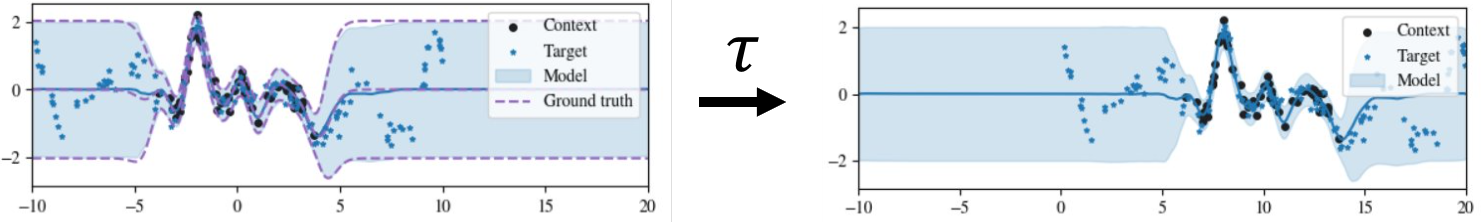
\includegraphics[width=0.9\textwidth]{./te.PNG}
	\caption{The Translation Equivariant property on a 1D dataset.}
	\label{fig:te}
\end{figure}


\autoref{fig:te} illustrates this property, when the input data on the left plot is shifted by a constant amount, the prediction should also shift by the same amount (right).

\begin{align}
	&f: \bm{x} \rightarrow (\bm{x}, \bm{\hat{y}}) \\
	&f: \bm{x} + \bm{c} \rightarrow (\bm{x} + \bm{c}, \bm{\hat{y}})
\end{align}

where $\bm{x}$ is the input and $\bm{\hat{y}}$ is the output and $\bm{c}$ is a constant shift in the input. This property allows the model to be more robust and generalize better to unseen data, particularly in the case of stationary data.


\textbf{Off-the-Grid Generalization}: \emph{The model should be able to work on off-the-grid data points}. Off-the-grid data points are the data points that are not in a regular gridded structure, for example, images that have missing pixel values are off-the-grid. Traditional models like Convolutional Neural Networks (CNNs) are not able to operate on off-the-grid data points since they require a regular structure to apply the convolution operation. By making the model off-the-grid generalizable, we can create models that can work on many types of data and easily handle missing data points. It also allows the model to generalize to regions of the input space that it has not seen during training. Tasks like image inpainting, where the model is required to fill in missing pixels in an image, can benefit from this property.

\todo{Add a figure to illustrate off-the-grid generalization}

Neural Processes (NPs) \cite{garnelo2018neural} are a class of models that satisfy the above properties. The framework undermining NPs is general purpose, and thus can be modified with a variety of neural network architectures. 

\section{Aims and Objectives}

In this work, we aim to implement and compare two different neural network architectures for Neural Processes, the first being based on a Convolutional Neural Network (CNN) called Convolutional Neural Processes (ConvNP) and the second being based on a Transformer architecture called Transformer Neural Processes (TNP). We aim to compare the two models on a variety of tasks and datasets to see how they perform in terms of generalization, scalability, and uncertainty estimation. 

Furthermore, we investigate how the TNP can be optimized to achieve better performance. We then investigate new Transformer architectures that have better computational efficiency compared to the original Transformer architecture. 

Our end goal is to develop a better understand of the properties of these models. We aim to figure out the best practices for using these models in different scenarios, where they perform well and where they do not. We also aim to understand the limitations of these models and how they can be improved.





\ifSubfilesClassLoaded{%
    \printbibliography{}
}{} 


\end{document}